\chapter{Analisi}

\section{Requisiti}

Il progetto si pone tre principali obiettivi:
\begin{itemize}
	\setlength\itemsep{0.8em}
	\item La generazione automatica di pacchetti di installazione multi-piattaforma \\ con \ac{jre} integrato
	\item La pubblicazione automatica di rilasci all'interno dell'\ac{aur}
	\item Lo sviluppo di una \ac{cli} per interagire con il simulatore
\end{itemize}
Con integrazione di un \ac{jre} si intende il supplemento di una \ac{jvm}, frequentemente ridotta di dimensioni, all'interno del pacchetto di installazione.
L'utente potrebbe non aver alcun \ac{jre} installato sul proprio dispositivo, oppure quello presente potrebbe essere obsoleto. Inserendo una macchina virtuale Java: si fornisce uno specifico ambiente di esecuzione eliminando potenziali problemi di compatibilità e si agevola la procedura di installazione per l'end-user.

\paragraph{Requisiti funzionali}

Le funzionalità richieste si possono classificare in due gruppi distinti: il primo contiene tutto ciò che concerne l'esperienza dell'utente finale, mentre il secondo descrive le funzionalità dal punto di vista degli sviluppatori e contributori di Alchemist. Di seguito il primo gruppo.
\begin{itemize}
	\item \textbf{Multi-piattaforma}: Alchemist deve essere installabile sui maggiori sistemi operativi in circolazione come Windows, MacOS e le principali distribuzioni Linux.
	\item \textbf{Usabilità}: il simulatore deve fornire un'interfaccia \ac{cli} autoesplicativa e completa, ossia che permetta l'utilizzo di tutte le sue funzionalità.
\end{itemize}

I requisiti del gruppo successivo sono accumunabili per il loro scopo, vale a dire l'automazione.

\begin{itemize}
	\item \textbf{Automazione dei pacchetti}: la generazione dei pacchetti di installazione deve essere automatica e configurabile
	\item \textbf{Automazione della distribuzione}: il rilascio di una nuova versione deve essere eseguita autonomamente fornendo i pacchetti come assets di GitHub e pubblicare l'aggiornamento nell'\ac{aur}.
	\item \textbf{Verifica funzionamento}: entrambi i processi descritti precedentemente devono essere corredati da verifiche del loro funzionamento e devono bloccare la procedura di rilascio nell'eventualità siano presenti errori.
\end{itemize}

\paragraph{Requisiti non funzionali}

\begin{itemize}
	\item Trattandosi Alchemist di un software in continuo sviluppo, è auspicabile l'utilizzo degli strumenti già impiegati all'interno del repository. \\ L'integrazione di nuovi applicativi deve essere eseguita solo se strettamente necessaria.
	\item Il tempo di esecuzione della pipeline non deve incrementare.
\end{itemize}

\section{Impacchettamento}

\section{Strumenti}

\subsection{Gradle}

Mentre in passato la produzione di artefatti (documentazione, pacchetti, eseguibili) era delegata a script costruiti dallo sviluppatore, in un progetto di grandi dimensioni è oggigiorno essenziale avvalersi di uno strumento di build automation. Come l'output di un programma deterministico non cambia per uno stesso input, la produzione di artefatti deve essere consistente e riproducibile riducendo al minimo l'intervento umano. 

Gradle è uno dei tanti strumenti disponibili, supporta diversi linguaggi di programmazione anche se risulta popolare nell'ambiente JVM come alternativa a Maven. Gli script Gradle possono utilizzare due differenti \ac{dsl}: Groovy o Kotlin. I \textit{task} sono l'unità minima di esecuzione e rappresentano un azione: come generare un JAR, eseguire dei test o produrre la documentazione. Mediante direttive come \textit{dependsOn} è possibile creare dipendenze tra processi, Gradle per orchestrare l'esecuzione dei task costruisce un grafo aciclico diretto (DAG) delle dipendenze. L'esecuzione di Gradle avviene in tre fasi distinte elencate di seguito.
\begin{enumerate}
	\item \textbf{Fase di inizializzazione}. In primo luogo Gradle crea un istanza di Settings che organizza l'architettura del progetto. Attraverso un file, di nome ``settings.gradle", lo sviluppatore stabilisce il progetto radice e tutti gli eventuali progetti figli. 
	\item \textbf{Fase di configurazione}. Successivamente tutti i file di configurazione ``build.gradle" (del progetto radice e tutti i sotto-progetti) vengono analizzati per costruire il grafo dei task.
	\item \textbf{Fase di esecuzione}. Infine, Gradle esegue i task richiesti considerando le dipendenze descritte nel grafo generato dalla fase precedente.
\end{enumerate}

\begin{figure}[H]
	\centering
	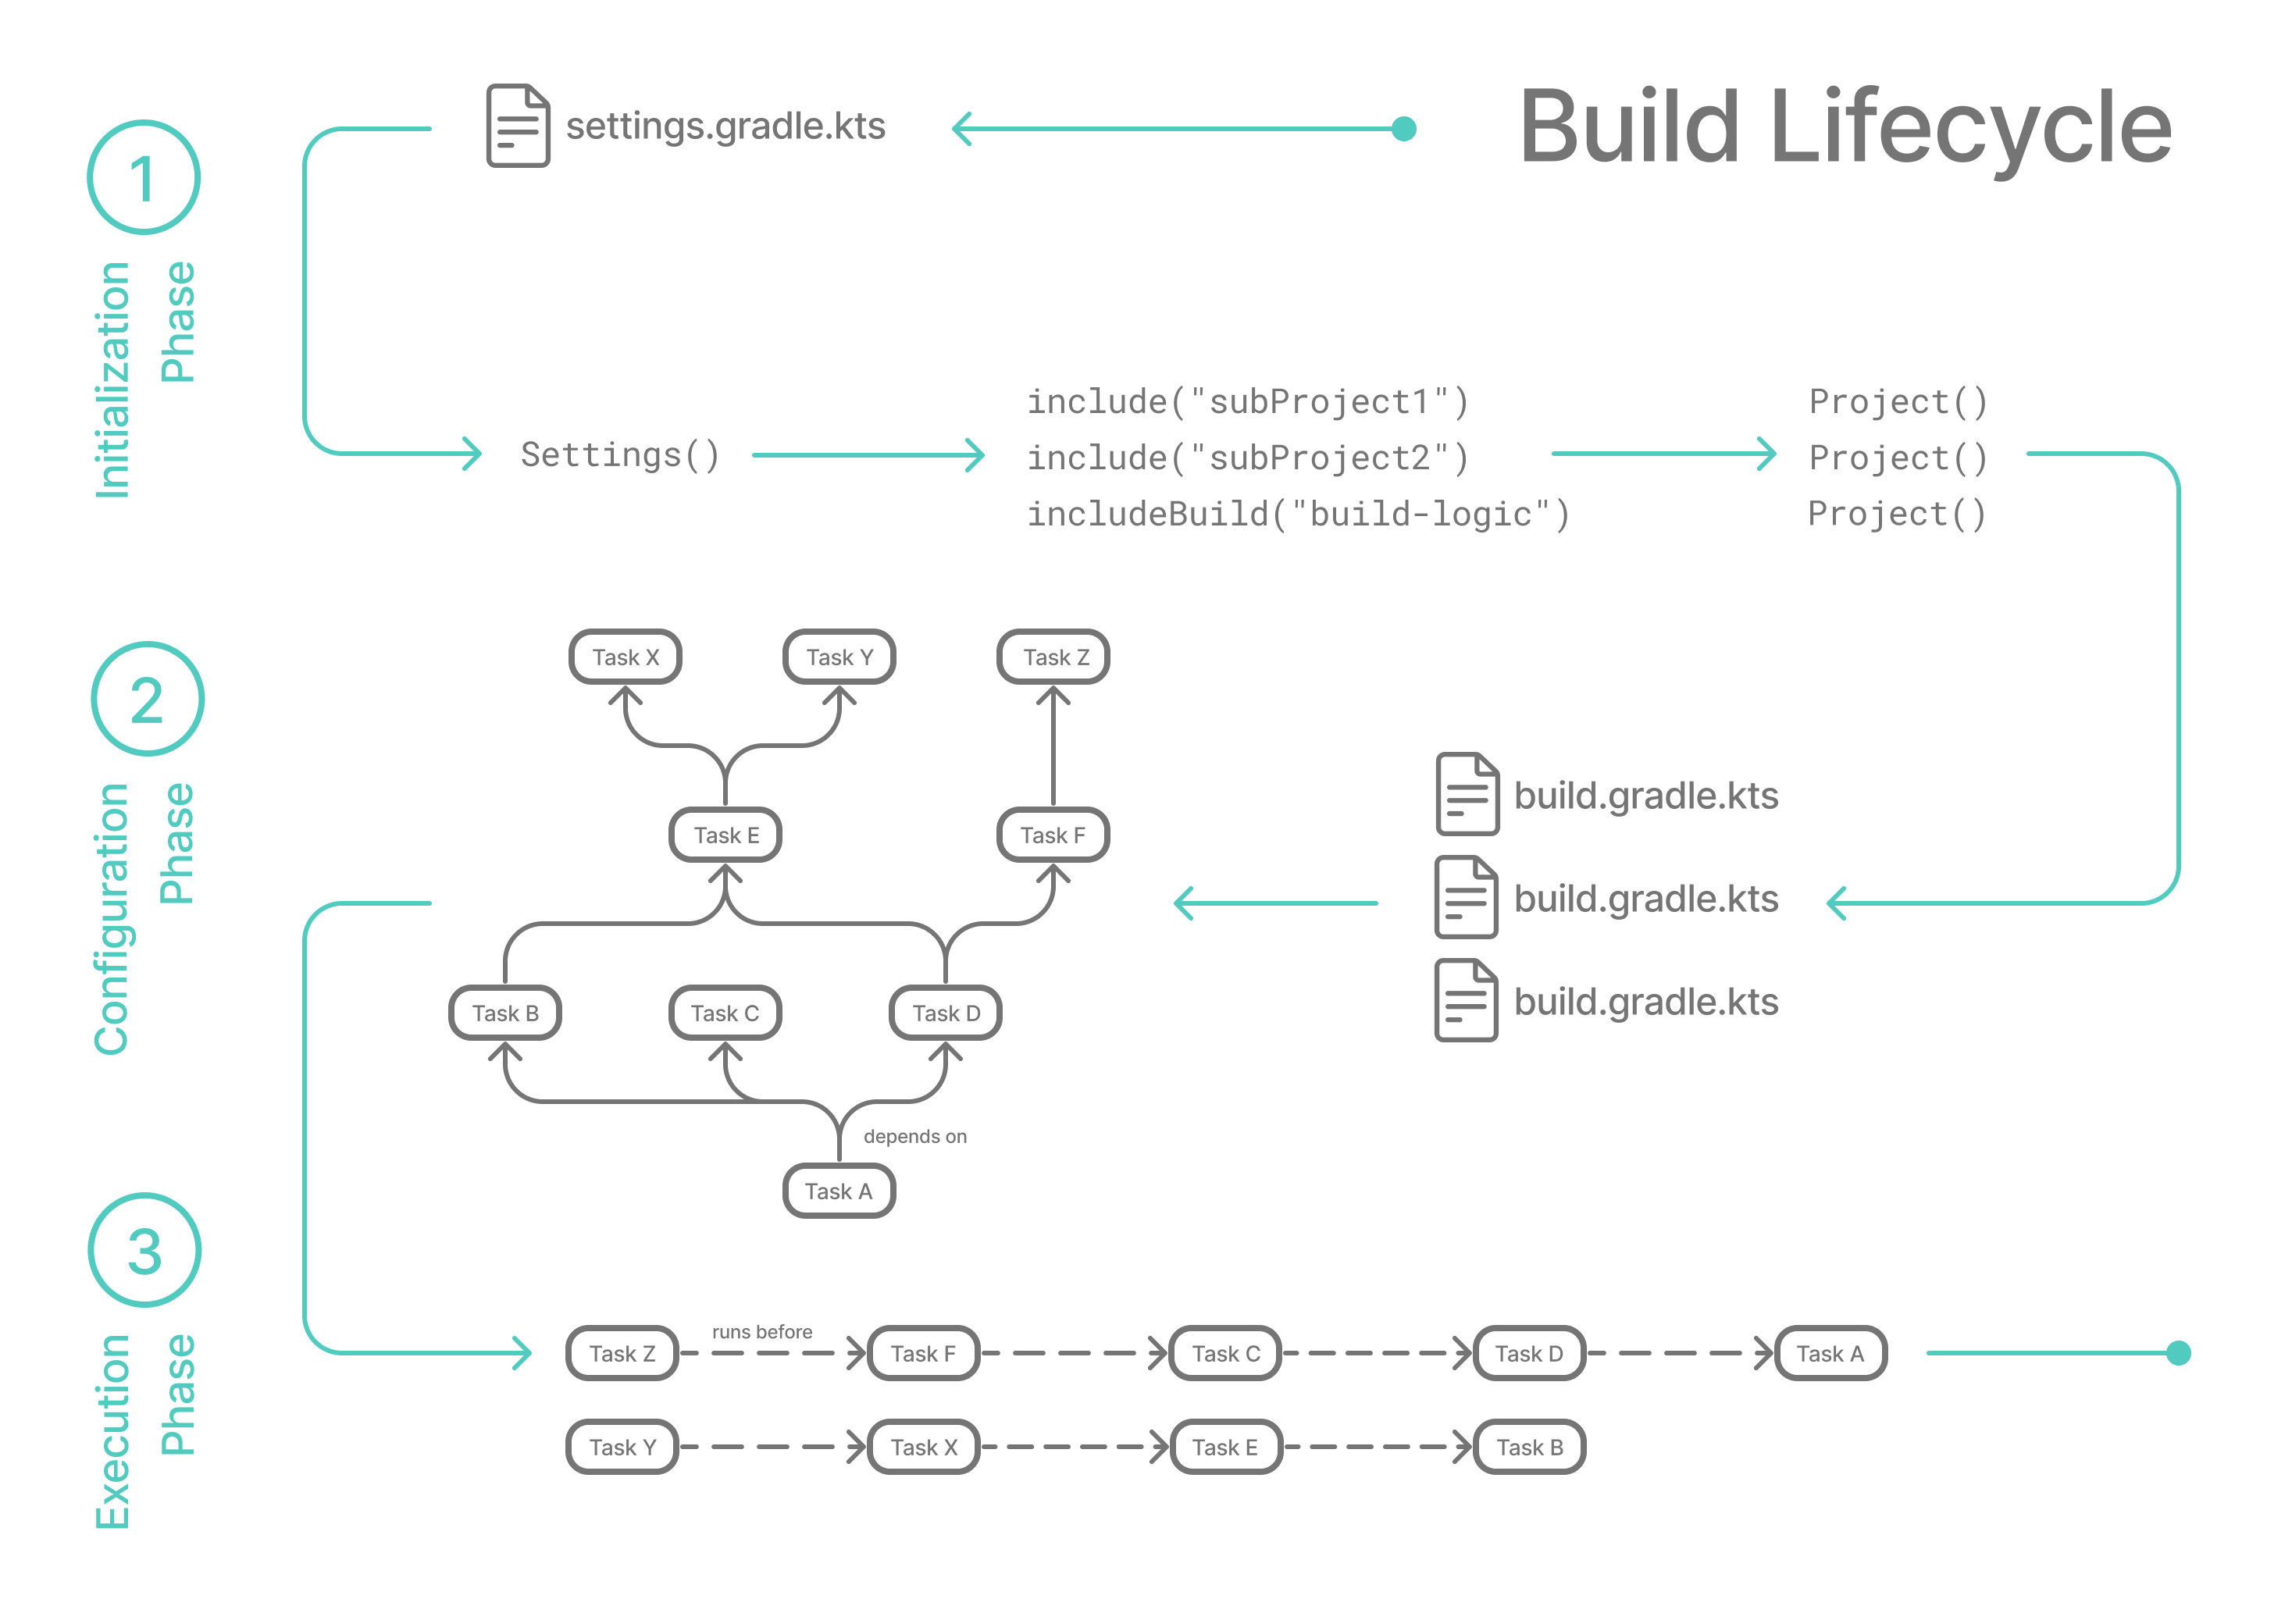
\includegraphics[width=.8\linewidth]{figures/gradle-build-lifecycle-example.png}
	\caption{Esempio di inizializzazione, configurazione ed esecuzione di una build Gradle}
	\label{fig:gradle-build-lifecycle}
\end{figure}
Un componente chiave sono i plugin, i quali consentono di estendere le funzionalità di Gradle: aggiungere nuovi task, estendere il modello con nuovi elementi \ac{dsl} ed applicare configurazioni specifiche all'intero progetto. La presenza di diversi plugin base e creati dalla comunità rende Gradle uno strumento versatile.
\paragraph{Analisi rispetto ai requisiti}
In considerazione dei requisiti di automazione, Gradle fornisce le funzionalità per soddisfare i requisiti di pacchettizzazione, distribuzione e verifica del funzionamento. L'utilizzo di un \ac{dsl} come Kotlin consente l'accesso ad un infinità di moduli per interagire ad alto livello con il sistema sottostante. L'approccio task-based inoltre permette di suddividere un macro-processo in più unità di esecuzione riutilizzabili da altri processi, garantendo tutti i vantaggi che la filosofia \ac{dry} fornisce.

\newpage
\subsection{GitHub Actions}

Tramite Gradle lo sviluppatore è in grado di eseguire procedure articolate come compilazione, test e dispiegamento utilizzando un semplice comando da \ac{cli}. \\ L'esecuzione di queste procedure richiede però l'intervento umano e non è sufficiente per garantire un flusso di integrazione e rilascio continuo. 

GitHub Actions è una piattaforma di \ac{cicd} disponibile per i repository ospitati su GitHub. Consente la configurazione ed esecuzione di pipeline personalizzate, i \textit{workflow}. Un workflow consiste in un insieme di \textit{job} eseguiti sequenzialmente o parallelamente all'interno di una macchina virtuale detta \textit{runner}. La piattaforma fornisce macchine virtuali per ogni sistema operativo (Windows, MacOS e Linux) con la possibilità di utilizzare container docker. GitHub in primo luogo è una piattaforma di code-sharing orientata allo sviluppo open source, una peculiarità della funzionalità Actions è la vasta gamma di eventi configurabili per avviare un workflow: dall'apertura di una pull-request, un commento o la creazione di un fork.

I workflow sono descritti in file YAML all'interno di una cartella specifica del repository. In primis si configura il nome del workflow e l'evento che origina l'esecuzione di esso, successivamente l'elenco dei job ed gli step che lo compongono. 

\begin{figure}[H]
	\centering
	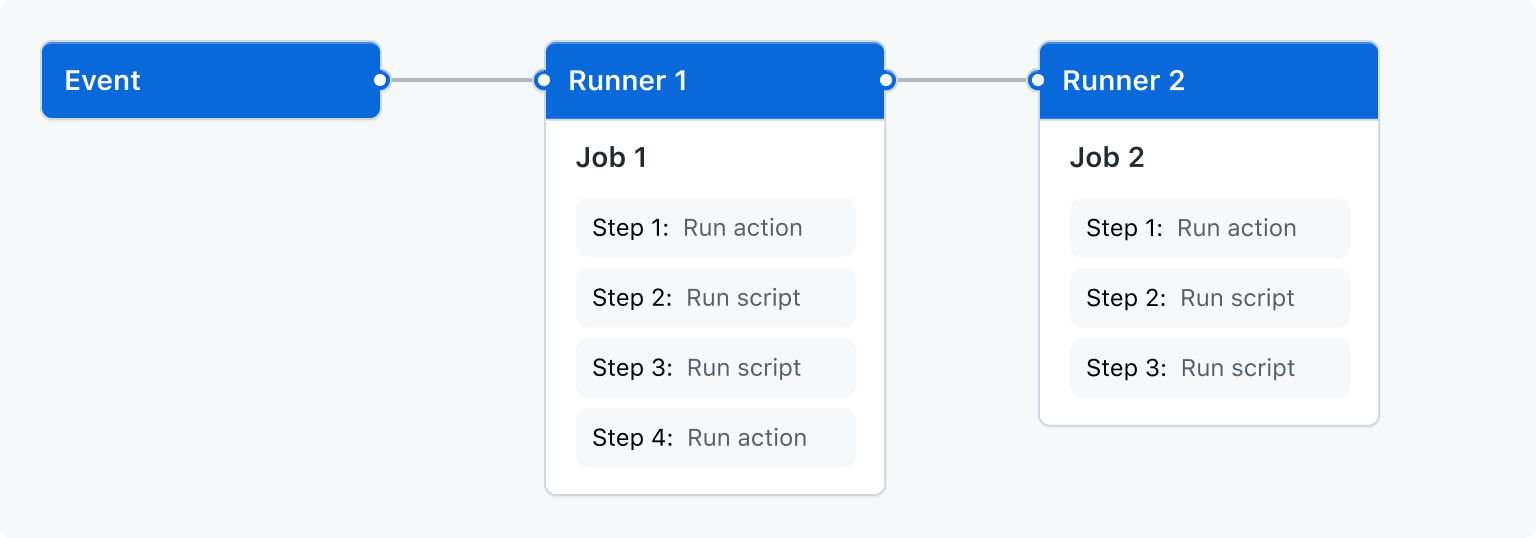
\includegraphics[width=.9\linewidth]{figures/overview-actions-simple.png}
	\caption{Sintesi dei componenti utilizzati su GitHub Actions ed esempio di un workflow \\ source: https://docs.github.com/en/actions/learn-github-actions/understanding-github-actions}
	\label{fig:github-actions-example}
\end{figure}

Uno step può presentare una lista di comandi eseguiti nella shell di riferimento (quella di default per il sistema operativo o un'altra se specificata) altrimenti ciò che dà il nome alla piattaforma: una action. Una action è un componente riutilizzabile che esegue un'attività particolare, esistono diverse azioni sviluppate dalla comunità e rese disponibili all'interno di un marketplace vasto. Per esempio una delle più diffuse è ``actions/checkout" che clona il repository del progetto nella cartella di lavoro corrente del runner.

\paragraph{Analisi rispetto ai requisiti}

La piattaforma di GitHub Actions ricopre un ruolo fondamentale nell'ambito dell'automazione: offre l'infrastruttura per l'esecuzione delle pipeline.

\subsection{Arch User Repository}

Nei sistemi operativi Linux il controllo dei componenti installati nella macchina è completamente delegato ai \textit{package manager}. Il \textit{package-management system} è un insieme di strumenti software che gestiscono i processi di installazione, aggiornamento, configurazione e rimozione di applicativi dal sistema. Spesso un pacchetto corrisponde ad un particolare programma o applicazione. Allo stesso tempo però esistono applicativi più complessi composti da più pacchetti correlati. Il sistema di gestione dei pacchetti opera attraverso tre componenti principali.

\begin{itemize}
	\item Un componente a basso livello che si occupa dell'installazione o rimozione dei pacchetti.
	\item Un componente ad alto livello il cui compito principale è quello di fornire un'interfaccia per la gestione dei pacchetti all'utente. Si occupa inoltre di risolvere le dipendenze e gestire le sorgenti (repository).
	\item I repository, ossia database pubblici contenenti i pacchetti ed i relativi meta-dati.
\end{itemize}

\begin{figure}[H]
	\centering
	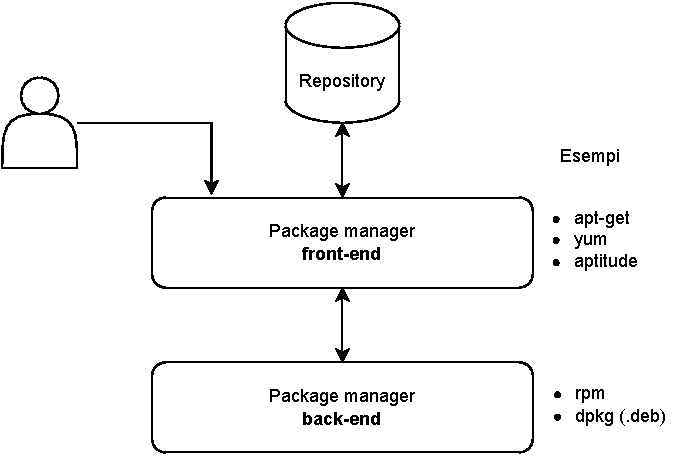
\includegraphics[width=.7\linewidth]{figures/package-managers.pdf}
	\caption{Struttura più diffusa dei sistemi di gestione di pacchetti}
	\label{fig:package-managers}
\end{figure}

\paragraph{Arch Linux} Una distribuzione importante nel vasto panorama dei fork Linux è Arch. Arch è una distribuzione Linux con architettura x86-64 creata seguendo la filosofia \ac{kiss}. È infatti rinomata per essere leggera, veloce, estremamente scalabile ed adattabile alle proprie esigenze. Data la sua natura minimalista, l'installazione iniziale non incorpora alcun strumento di configurazione automatica, nessun ambiente desktop e nessun altro strumento necessario all'avvio del sistema. Il sistema di gestione dei pacchetti si chiama \textit{pacman} ed a differenza dei concorrenti, opera sia a basso che ad alto livello. Un pacchetto non è altro che un file shell script denominato \textit{PKGBUILD} contenente le istruzioni necessarie a scaricare i sorgenti e compilarli attraverso un comando: \textit{makepkg}. La linearità dei file PKGBUILD rende la creazione di pacchetti alla portata di qualsiasi utente. \textbf{\ac{aur}} è una peculiarità di Arch che la distingue dalle altre distribuzioni. Si tratta di un repository di pacchetti in cui qualsiasi utente, anche non sviluppatore, può contribuire. 

\paragraph{Analisi rispetto ai requisiti}
Nell'ottica di soddisfare il requisito multi-piattaforma del progetto è necessario analizzare le piattaforme di destinazione per il simulatore. Mentre per Windows e MacOS esistono specifiche tipologie di pacchetti di installazione supportati ufficialmente, per Linux non esiste uno standard univoco. Tuttavia  i pacchetti RPM e DEB sono supportati dalla maggior parte delle distribuzioni, in particolare il primo è citato nella specifica ``Linux Standard Base". Il PKGBUILD di Arch supporta nativamente l'estrazione di sorgenti RPM e DEB, pertanto a fronte di questa analisi essi risultano la scelta più opportuna.

\subsection{Command Line Interface} 

CLI